\chapter{フェルミオンの質量：カイラリティ、湯川結合、マヨラナニュートリノ}

\lectureoverview{まずトイ模型である\(U(1)\)理論においてゲージボソンのヒッグス機構を再構築し、次にフェルミオンについて同様の問いを立てる。ディラック質量は左巻きと右巻きのカイラル場を混合するが、弱い相互作用はそれらに異なる電荷を割り当てるため、裸の質量項を禁じる。ヒッグス場への湯川結合は対称性を尊重する。ヒッグス場が真空期待値を獲得した後、同じ相互作用がフェルミオンの質量と測定可能なヒッグス--フェルミオン結合になる。最後の部分ではこの論理をニュートリノ質量、可能な重い保護されていない粒子、宇宙線の運動学、相対論的慣性、重力へと展開する。}

冒頭の復習の目的は、単に前回の講義を繰り返すことではない。そこから一つのアイデアを、フェルミオンに持ち越せる形で取り出す必要がある。すなわち、質量とはゼロ運動量における励起の非ゼロエネルギーである。場にとって、ゼロ運動量とは無限の波長、つまりどこでも同じ変位を意味する。微分のみの理論は一様な変位を検出できない。微分を含まない項はそれを検出できる。

\section{ゲージボソンの話を一通り}

\subsection{微分のエネルギーと質量のないベクトル}

模型のゲージ場は\(A_\mu\)であり、場の強さは
\begin{equation}
  F_{\mu\nu}
  =\partial_\mu A_\nu-\partial_\nu A_\mu .
  \label{eq:l09-field-strength}
\end{equation}
である。黒板ではゲージ運動項を模式的に\(F^2\)と書く。標準的な規格化では
\begin{equation}
  \mathcal L_{\mathrm{gauge}}
  =-\frac14 F_{\mu\nu}F^{\mu\nu}.
  \label{eq:l09-gauge-kinetic}
\end{equation}
である。

\begin{figure}[htbp]
\centering
\includegraphics[width=0.72\textwidth]{lecture_09_figure_02.png}
\caption{場の強さの定義と、ゲージ場の微分のエネルギーに対する黒板の\(F^2\)という略記。}
\lectureframe{00:02:39}
\label{fig:l09-field-strength-board}
\end{figure}

\eqref{eq:l09-gauge-kinetic}における\(A_\mu\)のすべての出現は微分されている。したがって、
\begin{equation}
  A_\mu(x)\longmapsto A_\mu(x)+c_\mu,
  \qquad \partial_\nu c_\mu=0,
\end{equation}
は\(F_{\mu\nu}\)を変えない。よって一様なベクトルポテンシャルは場の強さのエネルギーを要しない。講義の言葉では、ゼロ運動量モードにはギャップがなく、ゲージボソンは質量をもたない。

この\(U(1)\)場は意図的に単純化した代役である。物理的な目標は電磁光子ではなく\(W^\pm\)と\(Z\)である。破れていない電磁対称性は光子を質量のないままにし、破れた電弱対称性は弱いゲージボソンに質量を与える。

\subsection{ヒッグスの半径を凍結する}

電荷をもつ複素スカラーを導入し、極形式で書く。
\begin{equation}
  \phi(x)=\rho(x)e^{i\alpha(x)}.
\end{equation}
そのメキシカンハット型ポテンシャルは非ゼロ半径の円上で最小化される。その半径を\(f\)と呼ぶと、動径方向は比較的硬い。最初の一通りではそれを凍結し、位相のみを保持する：
\begin{equation}
  \phi(x)\simeq f e^{i\alpha(x)}.
  \label{eq:l09-frozen-higgs}
\end{equation}

\begin{figure}[htbp]
\centering
\includegraphics[width=0.72\textwidth]{lecture_09_figure_03.png}
\caption{凍結されたヒッグス半径、その共変微分、および復習で用いた小さな破れたポテンシャルのスケッチ。}
\lectureframe{00:06:42}
\label{fig:l09-frozen-board}
\end{figure}

規約
\begin{equation}
\begin{aligned}
  D_\mu&=\partial_\mu+igA_\mu,
  \\
  \phi&\longmapsto e^{i\theta}\phi,
  \\
  A_\mu&\longmapsto A_\mu-\frac1g\partial_\mu\theta .
\end{aligned}
  \label{eq:l09-gauge-convention}
\end{equation}
を選ぶ。講義では\(g\)を省略するが、それを可視のままにしておくと次元と最終的な質量が透明になる。凍結された場に作用させると
\begin{align}
  D_\mu\phi
  &=(\partial_\mu+igA_\mu)f e^{i\alpha}
  \notag\\
  &=i\bigl(\partial_\mu\alpha+gA_\mu\bigr)
    f e^{i\alpha}.
  \label{eq:l09-covariant-frozen}
\end{align}
となる。複素共役を掛けると位相が消え、また\(i\)掛ける\(-i\)が\(+1\)になる：
\begin{equation}
  |D_\mu\phi|^2
  =f^2
   \bigl(\partial_\mu\alpha+gA_\mu\bigr)
   \bigl(\partial^\mu\alpha+gA^\mu\bigr).
  \label{eq:l09-frozen-square}
\end{equation}

\begin{classroomqa}
\audiencequestion{微分が\(i\)の因子を生み出したので、共変微分の二乗は負符号をもつべきだろうか？
\lecturetimestamp{00:07:39}}
\lecturerresponse{いいえ。運動項は複素共役との積である。一方の因子が\(i\)を寄与し、他方が\(-i\)を寄与し、\(i(-i)=1\)となる。\(D_\mu\)の符号規約は一貫して逆にしてもよいが、対応するエネルギー表式において絶対値の二乗は正である。}
\end{classroomqa}

\eqref{eq:l09-frozen-square}の組み合わせはそれ自体がシフトされたゲージ場である。\(\theta=-\alpha\)を選び、スカラーの位相が消えるようにして、
\begin{equation}
  A'_\mu=A_\mu+\frac1g\partial_\mu\alpha .
  \label{eq:l09-unitary-gauge-field}
\end{equation}
と定義する。すると
\begin{equation}
  |D_\mu\phi|^2=g^2f^2 A'_\mu A'^\mu .
  \label{eq:l09-vector-mass-term}
\end{equation}
となる。新しい項は\(A'_\mu\)の微分を含まない。一様な場は今やエネルギーを蓄えるので、ゼロ運動量のベクトルモードにはギャップが生じる。

\begin{figure}[htbp]
\centering
\includegraphics[width=0.72\textwidth]{lecture_09_figure_04.png}
\caption{位相が吸収された後にゲージボソンの質量を示す\(f^2A^2\)の項を黒板から取り出す。}
\lectureframe{00:10:31}
\label{fig:l09-vector-mass-board}
\end{figure}

正準的なスカラーの規格化では
\(\phi=(f+h)e^{i\pi/f}/\sqrt2\)
と書く。得られたベクトル項を
\(\tfrac12m_A^2A_\mu A^\mu\)
と比較すると、このアーベル模型において
\begin{equation}
  m_A=gf
  \label{eq:l09-abelian-vector-mass}
\end{equation}
が得られる。講義では規格化因子を省略し、ベクトルの質量は\(f\)によって決まると要約する。

位相モードは何の説明もなく消えたわけではない。ゲージ化する前は、それは質量のないゴールドストーンボソンであった。ゲージ化した後は、質量をもつベクトル粒子に必要な縦偏極を供給する。一時的に凍結した動径方向の揺らぎは、物理的なヒッグス励起として残る。

\subsection{なぜ微分を含まない項が質量を意味するのか}

\begin{classroomqa}
\audiencequestion{なぜ\(A'^2\)項は単なる別の相互作用ではなく質量として数えられるのか。\lecturetimestamp{00:13:10}}
\lecturerresponse{質量とは静止エネルギーである。場について言えば、静止した粒子はゼロ運動量・無限波長モードの量子である。微分項は静的で一様な変位にエネルギーを与えないが、\(m_A^2A'^2\)は与える。この非ゼロのゼロ運動量エネルギーが静止エネルギーのギャップである。}
\end{classroomqa}

講義はこの主張を三つの力学的類推を通して展開する。

\begin{itemize}
  \item 結晶では、ゆっくり変化する変位は弾性エネルギーを要する。隣接原子が異なる変位を受けるからである。剛体並進はすべての原子を一緒にずらし、内部エネルギーを要しない。したがって音響フォノンはギャップレスである。
  \item 理想的な回転対称磁石では、空間的に変化するスピン方向は交換エネルギーを要するが、すべてのスピンを一緒に回転させても要しない。対応する長波長スピン波はギャップレスである。
  \item プラズマでは、電子流体を正の背景に対してずらすと、一様な相対変位であっても電荷分離と復元電場が生じる。結果として生じるプラズモンはゼロ波数で非ゼロの振動数をもつ。
\end{itemize}

ヒッグス化されたゲージ場は第三の例のように振る舞う。対称性の破れた媒質は、そうでなければ無コストの一様変位に抵抗する。

\begin{classroomqa}
\audiencequestion{ゲージ場が導入される前、位相\(\alpha\)はすでに振動していなかったのか。\lecturetimestamp{00:18:24}}
\lecturerresponse{振動していた。そのエネルギーは\(f^2(\partial_\mu\alpha)^2\)に比例していた。場所ごとに変化する位相は勾配エネルギーをもち伝播できるが、一様な位相の変化は何のコストも要しない。まさにこれが質量ゼロのゴールドストーンモードである。}
\end{classroomqa}

\begin{classroomqa}
\audiencequestion{微分には時間微分が含まれる。格子全体を実際に動かしたり場全体を変化させたりすることは運動エネルギーを運ばないのか。\lecturetimestamp{00:22:18}}
\lecturerresponse{運ぶ。比較は静的配置の間、または任意にゆっくり準備された配置の間で行われる。非ゼロの速度で並進する格子は運動エネルギーをもつ。質量のテストは、配置が静止し空間的に一様であるときにもエネルギーをもつかどうかを問う。}
\end{classroomqa}

\section{実験的手がかり：弱い相互作用は左と右を区別する}

講義は次に電子、ミューオン、クォークに移る。それらの質量もヒッグス場に由来するが、機構は異なって見える。フェルミオンの質量は二次のベクトル項ではないからである。それは二つのカイラル場の間の結合である。

\subsection{ベータ崩壊におけるパリティの破れ}

弱い相互作用がパリティを破るという経験的事実から始める。量子電磁力学と量子色力学は過程とその鏡像を同じように扱う。弱い相互作用はそうではない。中性子のベータ崩壊では、\begin{equation}
  n\longrightarrow p+e^-+\bar\nu_e,
  \label{eq:l09-beta-decay}
\end{equation}
荷電カレント相互作用によって選ばれる高エネルギー電子は左巻きのヘリシティをもつ。すなわちスピンが運動量と逆向きである。対応する反ニュートリノは逆のヘリシティをもつ。

超相対論的粒子について、ヘリシティを次で定義する。
\begin{equation}
  h=\frac{\bm S\cdot\bm p}{|\bm S|\,|\bm p|}.
\end{equation}
運動量に平行なスピンは\(h=+1\)、反平行なスピンは\(h=-1\)である。弱い相互作用は左カイラル電子場と左カイラルニュートリノ場に結合し、右カイラル電子場には同じようには結合しない。\editorialnote{講義は当初、高エネルギーで視覚的に直観的なため、ヘリシティの意味で左右の巻きを使う。ゲージ電荷は実際にはカイラリティに作用する。それは\(P_L=(1-\gamma^5)/2\)と\(P_R=(1+\gamma^5)/2\)によって選ばれるローレンツ表現のラベルである。質量ゼロの粒子では、粒子についてカイラリティとヘリシティは一致する。質量をもつ粒子では一致しない。}

完全な\(SU(2)_L\times U(1)_Y\)の記帳なしに障害を明らかにするため、\(U(1)\)という偽の世界を想像し、そこでは\(\psi_L\)だけが関連する電荷を運ぶとする。
\begin{equation}
  \psi_L\longmapsto e^{i\theta}\psi_L,
  \qquad
  \psi_R\longmapsto\psi_R .
  \label{eq:l09-chiral-toy-charge}
\end{equation}
これは電磁気学ではない。実際の左カイラル電子と右カイラル電子は同じ電荷を運ぶ。これは弱い相互作用の戯画であり、そこでは二つのカイラリティが異なる電弱表現に属する。

\begin{classroomqa}
\audiencequestion{同じ左--右の非対称性はクォークにも当てはまるか。\lecturetimestamp{00:31:50}}
\lecturerresponse{当てはまる。適切な弱多重項とハイパーチャージを用いる。左カイラルアップ型およびダウン型クォークは弱二重項を形成するが、右カイラル場は弱一重項である。したがってそれらのヒッグス結合は電子のものと同じ構造的問題に直面する。}
\end{classroomqa}

\section{ディラック質量は左--右混合である}

\subsection{四成分方程式から二つのワイル方程式へ}

ディラック波動関数は4つの成分をもつ。大まかに言えば、2つはスピンを記述し、2つは正エネルギー解と負エネルギー解を区別する。後者は反粒子の自由度として再解釈される。ハミルトニアン形式では、
\begin{equation}
  i\frac{\partial\Psi}{\partial t}
  =\left(-i\bm\alpha\cdot\bm\nabla+m\beta\right)\Psi .
  \label{eq:l09-dirac-hamiltonian}
\end{equation}
行列\(\alpha_i\)と\(\beta\)は、エネルギー、運動量、質量の間の相対論的関係を表す。

\begin{figure}[htbp]
\centering
\includegraphics[width=0.74\textwidth]{lecture_09_figure_05.png}
\caption{黒板にはまずディラック方程式が書かれ、次にそれが結合した左手系と右手系の方程式に分けられる。}
\lectureframe{00:40:30}
\label{fig:l09-dirac-board}
\end{figure}

カイラル基底は\(m\)の役割を明示する。
\(\sigma^\mu=(1,\bm\sigma)\)および
\(\bar\sigma^\mu=(1,-\bm\sigma)\)とすると、
\begin{align}
  i\bar\sigma^\mu\partial_\mu\psi_L&=m\psi_R,
  \label{eq:l09-weyl-left}\\
  i\sigma^\mu\partial_\mu\psi_R&=m\psi_L.
  \label{eq:l09-weyl-right}
\end{align}
\(m=0\)では、方程式は独立である。すなわち、左巻きカイラル場と右巻きカイラル場は互いに影響を与え合うことなく伝播できる。\(m\neq0\)では、それぞれが他方の源として現れる。これが、ディラック質量が左と右を混合するという正確な意味である。

サスキンドはこれを、フェルミオンが左と右の間を振動すると表現する。この言葉は結合を捉えているが、点粒子が行ったり来たり反転するという文字通りの古典的描像に押し込めるべきではない。正確な記述は、結合した場の方程式
\eqref{eq:l09-weyl-left}--\eqref{eq:l09-weyl-right}
である。

\begin{classroomqa}
\audiencequestion{黒板上の2つの方程式における\(i\)の因子と符号は整合しているか。\lecturetimestamp{00:41:10}}
\lecturerresponse{黒板上では行ごとに整合しているわけではない。素早い導出の際に、\(i\)が一貫性なく外に括り出された。信頼できる内容は結合のパターンである。方程式\eqref{eq:l09-weyl-left}と
\eqref{eq:l09-weyl-right}は、1つの標準的で整合した規約を与える。}
\end{classroomqa}

\subsection{なぜ弱い対称性が裸の質量を禁じるのか}

ラグランジアンにおける対応するディラック質量項は
\begin{equation}
  \mathcal L_m
  =-m\bar\psi\psi
  =-m\left(\bar\psi_L\psi_R+\bar\psi_R\psi_L\right).
  \label{eq:l09-bare-dirac-mass}
\end{equation}
である。おもちゃの変換\eqref{eq:l09-chiral-toy-charge}の下で、
\begin{equation}
  \bar\psi_L\psi_R\longmapsto
  e^{-i\theta}\bar\psi_L\psi_R,
  \qquad
  \bar\psi_R\psi_L\longmapsto
  e^{i\theta}\bar\psi_R\psi_L.
\end{equation}
どちらの項も不変ではない。したがって、直接的な左--右の混合係数\(m\)は、対称性の破れの前には禁じられている。

電磁気学だけではこの問題は生じない。なぜなら\(\psi_L\)と
\(\psi_R\)は同じ電荷をもつからである。障害は、両者の弱い量子数の違いから生じる。

\subsection{カイラリティの微妙さを露わにするヘリシティの問い}

ここで講義は、直感的な利き手の描像をいくつかの角度から検証する。これらの問いは本筋から外れた問題ではない。ヘリシティがどこで有用であり、どこでカイラリティに取って代わられなければならないかを正確に明らかにする。

\begin{classroomqa}
\audiencequestion{もし弱い相互作用が電子の両方のヘリシティを等しく放出するなら、世界はどのようになるだろうか。\lecturetimestamp{00:42:12}}
\lecturerresponse{その過程から直ちにパリティ非対称性が消えるだろう。しかし、実際の電弱理論はカイラルである。すなわち、荷電弱相互作用を担うのは左巻きカイラル二重項だけである。なぜ自然がその構造を選んだのかについてのより完全な説明は、講義では後回しにされる。}
\end{classroomqa}

\begin{classroomqa}
\audiencequestion{電子のスピンが鉛直に準備され、その後電子が水平に加速されるとする。それは左巻きか右巻きか。\lecturetimestamp{00:42:44}}
\lecturerresponse{運動量に横向きのスピン状態は、2つのヘリシティの重ね合わせである。ヘリシティが確定するのは、スピンが運動量に平行か反平行のときだけである。それにもかかわらず、弱いカイラル射影演算子は場に対して明確に定義される。}
\end{classroomqa}

質量をもつ粒子は、スピンを反転させることなく、静止するまで減速され、反対方向に加速されうる。そのときヘリシティは符号を変える。質量のない粒子は、ローレンツブーストによって追い越されたり静止させられたりすることはできないので、そのヘリシティは固有ブーストの下で不変である。このことが、ただ1つの物理的ヘリシティしかもたない種は質量がゼロでなければならないという講義の主張を動機づける。より正確な場の理論の主張は、ローレンツ不変なディラック質量は両方のカイラリティを必要とするということである。

\begin{classroomqa}
\audiencequestion{円偏光した光子は、鏡で反射して、決して静止することなく方向を反転できる。これはヘリシティの議論と矛盾するか。\lecturetimestamp{00:45:28}}
\lecturerresponse{いいえ。鏡は角運動量を交換し、伝播方向を反転させうる外部系である。反射過程は光子を追い越すローレンツブーストではない。チャネルが存在するかどうかは、許される偏光状態と物質の境界条件にも依存する。}
\end{classroomqa}

\begin{classroomqa}
\audiencequestion{普通の電子ビームは一方の利き手を含むのか、それとも両方を含むのか。\lecturetimestamp{00:46:10}}
\lecturerresponse{一般には両方である。質量をもつ電子状態は両方のカイラル成分を含み、非偏光ビームは両方のヘリシティを含む。特殊な線源は、大きなヘリシティ非対称性をもつ偏光ビームを生成できる。}
\end{classroomqa}

\begin{classroomqa}
\audiencequestion{ビームはそのスピンとは独立に集束できるのか、それとも磁場が2つの偏極を分離するのか。\lecturetimestamp{00:46:29}}
\lecturerresponse{通常の位置集束はスピンにほとんど鈍感でありうるが、磁気モーメントは磁場勾配と結合する。したがって、スピン選択的源、Stern--Gerlach的な勾配、加速器のスピンダイナミクスによって、偏極を準備したり分離したりできる。}
\end{classroomqa}

\begin{classroomqa}
\audiencequestion{左と右の間の弱い差異は単なる偶然なのか。\lecturetimestamp{00:48:13}}
\lecturerresponse{現在の講義では、それは標準模型に組み込まれた実験的事実である。あまりに体系的であり、気まぐれな偶然のようには感じられないが、標準模型自体はカイラル電荷の完全なパターンをより深い原理から導出してはいない。}
\end{classroomqa}

\section{湯川構成}

\subsection{ヒッグスに欠けている電荷を担わせる}

対称性は数値的な質量を禁じるが、欠けている変換位相を供給する場との相互作用は許す。複素スカラーを導入して
\begin{equation}
  \phi\longmapsto e^{i\theta}\phi,
  \qquad
  \phi^\dagger\longmapsto e^{-i\theta}\phi^\dagger.
  \label{eq:l09-scalar-charge}
\end{equation}
すると
\begin{equation}
  \mathcal L_Y
  =-y\,\bar\psi_L\phi\psi_R
   -y^*\,\bar\psi_R\phi^\dagger\psi_L
  \label{eq:l09-yukawa-lagrangian}
\end{equation}
はゲージ不変である。第1項では、
\(\bar\psi_L\)が\(e^{-i\theta}\)を寄与し、\(\phi\)が
\(e^{i\theta}\)を寄与する。位相は相殺する。第2項はそのエルミート共役である。

等価に、カイラル方程式は場に依存する混合を獲得する：
\begin{align}
  i\bar\sigma^\mu D_\mu\psi_L
    &=y\phi\psi_R,
  \label{eq:l09-yukawa-eom-left}\\
  i\sigma^\mu\partial_\mu\psi_R
    &=y^*\phi^\dagger\psi_L.
  \label{eq:l09-yukawa-eom-right}
\end{align}

\begin{figure}[htbp]
\centering
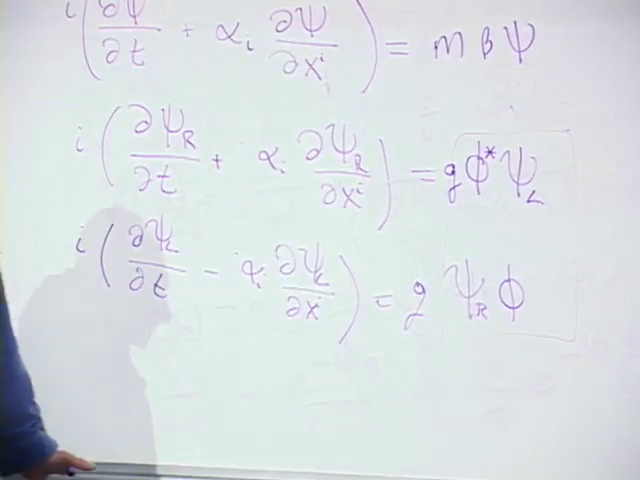
\includegraphics[width=0.76\textwidth]{lecture_09_figure_06.png}
\caption{右辺の裸の質量は荷電スカラー場に置き換えられた。黒板の正確な符号は概略的であり、不変な構造は\eqref{eq:l09-yukawa-lagrangian}に与えられている。}
\lectureframe{00:51:30}
\label{fig:l09-yukawa-board}
\end{figure}

対称性の破れの前では、これは質量ではなく相互作用である。右巻きカイラルフェルミオンは、電荷を釣り合わせるのに必要なスカラー量子を放出または吸収するときにのみ、左巻きカイラルフェルミオンになりうる。係数\(y\)は湯川結合であり、ゲージ電荷\(g\)ではない。

\begin{classroomqa}
\audiencequestion{単に\(\phi\)と
\(\phi^\dagger\)を2つの方程式の右辺に置くことは正当か。
\lecturetimestamp{00:51:55}}
\lecturerresponse{それらの変換位相が不整合を修復するまさにその理由で正当である。決定的なテストは方程式の見た目の形ではなく、相互作用
\(\bar\psi_L\phi\psi_R+\mathrm{h.c.}\)のゲージ不変性である。}
\end{classroomqa}

\subsection{真空が相互作用を質量に変換する}

ここで\(\phi\)をヒッグス場と同一視し、それが非零の真空の大きさに落ち着くようにする。講義の簡略化された規格化では、
\begin{equation}
  \phi\simeq f,
\end{equation}
したがって\eqref{eq:l09-yukawa-lagrangian}は
\begin{equation}
  \mathcal L_Y
  \supset
  -yf\,\bar\psi_L\psi_R
  -y^*f\,\bar\psi_R\psi_L .
\end{equation}
を含む。適切な場合には無害な位相の再定義の後、フェルミオン質量は
\begin{equation}
  m_f=yf.
  \label{eq:l09-lecture-fermion-mass}
\end{equation}
である。これはベクトルの結果\(m_A=gf\)のフェルミオン版である。弱ゲージボソンに縦偏極を供給するのと同じヒッグス真空が、左巻きと右巻きのフェルミオンを結びつけるのに必要な欠けている弱量子数を供給する。

標準的に規格化された標準模型の慣習では、
\begin{equation}
  H(x)=\frac1{\sqrt2}
  \begin{pmatrix}
    0\\ v+h(x)
  \end{pmatrix},
  \qquad v\simeq246\ \mathrm{GeV},
  \label{eq:l09-sm-higgs-vacuum}
\end{equation}
したがって
\begin{equation}
  m_f=\frac{y_fv}{\sqrt2}.
  \label{eq:l09-sm-fermion-mass}
\end{equation}
講義の\(f\)と従来の\(v/\sqrt2\)は、この規格化の選択だけが異なる。

\begin{classroomqa}
\audiencequestion{積\(yf\)だけがフェルミオン質量であるなら、結合\(y\)と真空スケール\(f\)を別々に決定するにはどうすればよいのか。
\lecturetimestamp{00:55:36}}
\lecturerresponse{弱ゲージボソン質量は、ゲージ結合がわかれば真空スケールを決定する。フェルミオンの測定された質量は、次にその湯川結合を決定する。完全な理論では、
\(m_W=gv/2\)、\(m_Z=v\sqrt{g^2+g'^2}/2\)、そして
\(y_f=\sqrt2m_f/v\)である。}
\end{classroomqa}

\begin{classroomqa}
\audiencequestion{弱ボソン質量はおよそ\(900\ \mathrm{GeV}\)か。
\lecturetimestamp{00:57:43}}
\lecturerresponse{いいえ。講義は直ちにその言い間違いをおよそ\(90\ \mathrm{GeV}\)に訂正する。より正確には、
\(m_W\simeq80\ \mathrm{GeV}\)および\(m_Z\simeq91\ \mathrm{GeV}\)であり、一方、根底にある真空スケールは\(v\simeq246\ \mathrm{GeV}\)である。}
\end{classroomqa}

\subsection{1つの真空スケール、多くの湯川結合}

すべての荷電フェルミオン種はそれぞれ独自の湯川結合を持つ：
\begin{equation}
  m_i=y_i f
  \qquad\text{(lecture normalization)}.
  \label{eq:l09-mass-family}
\end{equation}

\begin{figure}[htbp]
\centering
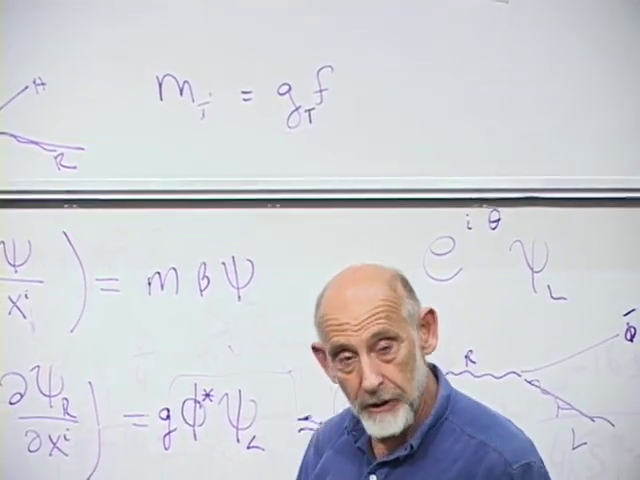
\includegraphics[width=0.76\textwidth]{lecture_09_figure_08.png}
\caption{黒板は種依存性を\(m_i=g_i f\)と要約している。そこに書かれた\(g_i\)は、ここで\(y_i\)と呼ばれる湯川結合である。}
\lectureframe{01:16:30}
\label{fig:l09-mass-family-board}
\end{figure}

電子について、講義は
\begin{equation}
  y_e\sim\frac{0.5\ \mathrm{MeV}}{10^2\ \mathrm{GeV}}
  \sim10^{-5}.
\end{equation}
と見積もる。標準的な値\(v=246\ \mathrm{GeV}\)を用いると、より正確な
\(y_e\simeq2.9\times10^{-6}\)が得られる。トップクォークは反対の端に位置する：
\begin{equation}
  y_t=\frac{\sqrt2m_t}{v}\simeq1.
\end{equation}
したがって、ヒッグス機構はゲージ不変な質量がどのように存在しうるかを説明するが、\(y_i\)の間の巨大な階層性を説明するものではない。観測されたフェルミオン質量は、その階層性を測定された数値に翻訳するにすぎない。

\begin{classroomqa}
\audiencequestion{トップクォークは本当に1程度のユカワ結合を持つのか？\lecturetimestamp{00:59:09}}
\lecturerresponse{はい。その質量は電弱スケールと同程度であるため、その結合は電子のような微小な摂動論的数値ではない。現代的な規格化では\(y_t\)は1に近い。}
\end{classroomqa}

\subsection{物理的ヒッグス揺らぎの復元}

スカラー場を真空期待値に固定すると動径方向の励起が隠れてしまう。それを模式的
に復元すると：
\begin{equation}
  \phi(x)\simeq f+h(x).
\end{equation}
ユカワ因子は次のようになる：
\begin{equation}
  y\phi\simeq yf+yh=m_f+yh.
  \label{eq:l09-mass-plus-higgs}
\end{equation}

\begin{figure}[htbp]
\centering
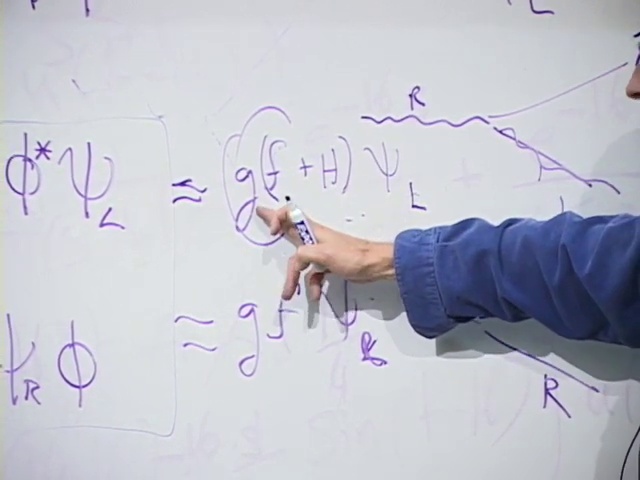
\includegraphics[width=0.76\textwidth]{lecture_09_figure_07.png}
\caption{この板書はユカワ項の中のヒッグス揺らぎを復元している：定数部分はフェルミオンの質量を生み出し、揺らぎの部分はヒッグスの放出または吸収を生み出す。}
\lectureframe{01:01:15}
\label{fig:l09-higgs-fluctuation-board}
\end{figure}

\eqref{eq:l09-mass-plus-higgs}の第一項は質量である。第二項はヒッグスボソンがフェルミオンに結合する頂点である。標準模型の標準的な記法では、
\begin{equation}
  \mathcal L_Y
  \supset
  -m_f\bar\psi\psi
  -\frac{m_f}{v}h\bar\psi\psi.
  \label{eq:l09-higgs-fermion-vertex}
\end{equation}
結合はフェルミオンの質量に比例する。運動学的条件、カラーの因子、位相空間、および競合するチャネルを考慮に入れた上で、したがってヒッグスはより重いフェルミオンにより強く結合する。

\begin{classroomqa}
\audiencequestion{結合定数それ自体は確率なのか？\lecturetimestamp{01:03:35}}
\lecturerresponse{それらは量子振幅に入る。単純な率はしばしば振幅の絶対値の二乗に比例し、したがって結合の二乗に比例するが、位相空間、スピン和、干渉、ループ、および複数の頂点も重要である。結合を確率と直接同一視すべきではない。}
\end{classroomqa}

\begin{classroomqa}
\audiencequestion{この議論はヒッグス場が1つだけであることを仮定しているのか？\lecturetimestamp{01:03:59}}
\lecturerresponse{それは1つの複素ヒッグス二重項を持つ最小標準模型を記述している。その4つの実成分のうち3つは\(W^\pm\)と\(Z\)に吸収され、1つの物理的な中性スカラーが残る。拡張模型はより多くの二重項や他のスカラー多重項を含むことができる。超対称模型は通常2つのヒッグス二重項を必要とし、したがって複数の物理的ヒッグス状態を含む。}
\end{classroomqa}

その歴史的な予想は今や実験と比較できる。
\editorialnote{この講義はヒッグス発見の前に収録された。ATLASとCMSは2012年にヒッグス様粒子を発表し、現在では\(125\ \mathrm{GeV}\)付近で測定されている。その観測された結合は、質量に比例する標準模型のパターンと概ね一致している。それが最も重い粒子へ優先的に崩壊するという記述は、常に運動学的な注意を伴う：オンシェルの\(t\bar t\)対は\(125\ \mathrm{GeV}\)ヒッグスに対して重すぎる。}

\section{反粒子、ビーム、およびカイラリティの意味}

ニュートリノに移る前に、クラスは反粒子と加速器ビームに関するいくつかの操作的な問いに戻る。

\begin{classroomqa}
\audiencequestion{左巻き電子の反粒子はどのようなヘリシティを持つのか？\lecturetimestamp{01:06:05}}
\lecturerresponse{左巻きカイラリティの電子場は、超相対論的極限において左ヘリシティの電子を消滅させ、右ヘリシティの陽電子を生成する。これは粒子対反粒子と、カイラリティ対ヘリシティを注意深く区別しなければならない箇所の一つである。}
\end{classroomqa}

\begin{classroomqa}
\audiencequestion{電子と陽電子を衝突させて\(Z\)ボソンを作ることはできるのか？\lecturetimestamp{01:07:13}}
\lecturerresponse{はい、それらの重心エネルギーが許されるチャネルと一致する場合にできる。電子--陽電子衝突型加速器は\(Z\)共鳴を非常に精密に研究した。電荷およびその他の量子数は過程全体を通じて保存される。}
\end{classroomqa}

\begin{classroomqa}
\audiencequestion{陽電子はすべて1つの特別な弱い過程を通じて生成されるのか？\lecturetimestamp{01:07:37}}
\lecturerresponse{いいえ。対生成は標準的な電磁気的な経路である。例えば、高エネルギーの電子は仮想光子を放出し、その光子は別の粒子の場の中で\(e^-e^+\)対を生成することができる。講義ではこれをファインマン図で描いている。}
\end{classroomqa}

\begin{classroomqa}
\audiencequestion{線形加速器はその電子の速度またはエネルギーを選別できるのか？\lecturetimestamp{01:09:24}}
\lecturerresponse{はい。加速場とタイミングがエネルギーの範囲を選別する。電子が超相対論的になると、その速度はすでに\(c\)に極めて近いので、追加の加速器エネルギーは主に運動量と全エネルギーを増加させ、速度を目に見えて増加させることはない。}
\end{classroomqa}

\begin{classroomqa}
\audiencequestion{加速器は1つの偏極のビームを準備できるのか？\lecturetimestamp{01:09:47}}
\lecturerresponse{はい、ただし技術的に困難である。スピン依存の源を用いて低エネルギーでスピン偏極電子を準備し、スピン歳差を制御しながらそれらを加速することができる。現代の衝突型加速器は、結果として得られるビーム偏極を完全に純粋なものとして扱うのではなく、定量的に評価する。}
\end{classroomqa}

\section{ニュートリノ質量とマヨラナの可能性}

\subsection{なぜニュートリノ質量が拡張を強制したのか}

元々の最小標準模型には左巻きカイラリティの中性子場しか含まれていなかったため、質量のない中性子が予言されていた。中性子振動は、少なくとも2つの中性子質量固有値が異なること、および中性子質量が非ゼロであることを示している。ただし、荷電フェルミオンの質量に比べればごくわずかである。

\begin{classroomqa}
\audiencequestion{中性子の質量はどれほど小さいのか、そしてその右巻き成分はどこにあるのか。\lecturetimestamp{01:10:38}}
\lecturerresponse{振動が決定するのは質量二乗差であり、絶対質量ではない。関連する分裂はおよそ\(0.009\ \mathrm{eV}\)および\(0.05\ \mathrm{eV}\)のスケールに対応する。ディラック的記述ではステライルな右巻きカイラリティの中性子が追加され、マヨラナ的記述では代わりに欠けているカイラリティを電荷共役中性子場に関連付ける。}
\end{classroomqa}

ディラック中性子の場合、新しい場\(\nu_R\)を追加し、湯川構成を繰り返す：
\begin{equation}
  \mathcal L_{\nu,\mathrm{Dirac}}
  =-y_\nu\bar L\,\widetilde H\,\nu_R+\mathrm{h.c.},
  \qquad
  m_\nu=\frac{y_\nu v}{\sqrt2}.
  \label{eq:l09-dirac-neutrino}
\end{equation}
必要な\(y_\nu\)は極めて小さい。

中性子が電荷を持たないため、別の論理的可能性がある。左巻きカイラリティの中性子は、逆のカイラリティを持つ自身の電荷共役と結合できる：
\begin{equation}
  \nu_L\longleftrightarrow(\nu_L)^c_R .
  \label{eq:l09-majorana-mixing}
\end{equation}
このようにして構成された質量固有状態はマヨラナフェルミオンである。すなわち、位相の規約を除けば、自身の反粒子である。同様の電子--陽電子混合は、厳密な電荷保存を破ることになるため禁止されている。

\begin{classroomqa}
\audiencequestion{なぜ粒子--反粒子混合は中性子では許されるが、電子では許されないのか。\lecturetimestamp{01:13:43}}
\lecturerresponse{電子と陽電子は逆の電荷を持つため、それらを同一の一粒子状態として混合する質量項は、破れていない電磁対称性を破ることになる。中性子は電気的に中性である。厳密に保存するレプトン数が中性子をその反粒子から区別しないならば、マヨラナ質量が許される。}
\end{classroomqa}

この名称は、この種の実フェルミオン表現を定式化し、1938年に失踪した若きイタリアの物理学者エットーレ・マヨラナにちなむ。講義はこの歴史的謎についてしばし留まる。彼の運命はついに確認されなかった。
\editorialnote{標準模型の活性中性子に対するゲージ不変なマヨラナ質量は、電弱対称性の破れ以前には繰り込み可能な裸の項ではない。低エネルギーでは、次元5のワインバーグ演算子\((LH)(LH)/\Lambda\)から、あるいは重いステライル中性子を介したシーソー機構を通じて生じうる。中性子がディラック粒子かマヨラナ粒子かは、実験的に未解決のままである。}

\section{なぜ身近なスペクトルは電弱スケール付近に集まるのか}

\subsection{共通スケールとその重要な但し書き}

\begin{classroomqa}
\audiencequestion{なぜヒッグス質量は弱スケールで到達可能と期待されたのか。\lecturetimestamp{01:14:48}}
\lecturerresponse{ヒッグスポテンシャルの曲率が動径方向のヒッグス質量を定め、同じ真空スケール\(f\)が\(W\)および\(Z\)の質量を定める。したがって、極端なスカラー自己結合がなければ、ヒッグス質量は弱スケールと同程度の広い桁になると期待された。観測された\(125\ \mathrm{GeV}\)の値は確かにそこにある。}
\end{classroomqa}

講義の印象的な要約は、最小標準模型の素粒子質量が1つの破れた真空に由来するということである：
\begin{align}
  m_W&=\frac12gv,\\
  m_Z&=\frac12\sqrt{g^2+g'^2}\,v,\\
  m_f&=\frac1{\sqrt2}y_fv.
  \label{eq:l09-electroweak-mass-summary}
\end{align}
無次元結合を固定したまま\(v\)が消えたならば、弱ゲージボソンと荷電素フェルミオンは質量がなくなったであろう。

その記述はその適用範囲を超えて拡大してはならない。光子とグルーオンは、破れていないゲージ対称性がそれらを保護するため質量のないままである。陽子と中性子の質量の大部分はQCD結合エネルギーであり、それらのクォークのヒッグス質量の和ではない。中性子質量は最小模型の拡張を必要とする。ヒッグス質量自体はスカラーポテンシャルに依存し、単に別の湯川質量ではない。

\subsection{質量が対称性の破れを待つ必要のない粒子}

新しいフェルミオンが同一のゲージ量子数を持つ左巻きおよび右巻きカイラリティ成分を持っていたとしよう。そのとき
\(\bar\Psi_L\Psi_R+\mathrm{h.c.}\)はすでにゲージ不変である。そのような\emph{ベクトル的}フェルミオンは、\(v\)とは無関係な裸の質量\(M\)を持ちうる：
\begin{equation}
  \mathcal L_{\mathrm{vectorlike}}
  =-M\bar\Psi\Psi.
  \label{eq:l09-vectorlike-mass}
\end{equation}
\(M\gg v\)に対する電弱対称性の障害はない。

これは講義の広い自然性の議論を動機付ける。ゲージ対称性またはカイラル対称性によって保護されている粒子は、ヒッグス真空がその保護を破るまで質量のないままであり、したがってそれらの質量は比較的小さいスケール\(v\)に結び付いている。そのような保護を持たない粒子は自然により重くてもよく、したがって観測される低エネルギー・スペクトルには存在しない。我々が見るものは選択効果かもしれない。すなわち、アクセス可能な粒子とは、その質量が電弱対称性の破れを待つことを強いられた粒子である。

\begin{classroomqa}
\audiencequestion{独立しており、はるかに大きな質量をもつ粒子は、現実には何の役割も果たさないのだろうか。\lecturetimestamp{01:19:39}}
\lecturerresponse{それらは生成が難しいため、通常の低エネルギー実験物理学ではほとんど役割を果たさないが、それでも高エネルギー史や宇宙論を形作る可能性はある。講義では、より重い隠れたスペクトルが最初に姿を現す可能性のある場所として、暗黒物質が挙げられている。}
\end{classroomqa}

2010の議論は、当時流行していた、弱いスケールかそれよりやや重い暗黒物質への期待を反映している。それは依然として有用な模型のクラスであって、確立した事実ではない。暗黒物質は重力的に検出されているが、その粒子としての正体と質量の起源は依然として不明である。

\section{結びの問い：宇宙線、慣性、重力、カイラリティ}

\subsection{質量は高い実験室エネルギーではない}

\begin{classroomqa}
\audiencequestion{宇宙線の質量はいくらか。
\lecturetimestamp{01:20:57}}
\lecturerresponse{宇宙線は陽子、原子核、電子、または光子であり得る。その不変質量は、その粒子または系の質量である。目を見張るのはその実験室エネルギーであり、最高エネルギーの事象ではおよそ\(10^{20}\)から\(10^{21}\ \mathrm{eV}\)に達する。高エネルギーは高い不変質量と同じではない。}
\end{classroomqa}

宇宙線が、ほぼ静止している標的粒子に衝突する。実験室エネルギー\(E\gg m_p\)の入射陽子に対して、
\begin{equation}
  s=(p_1+p_2)^2
  \simeq2m_pE+2m_p^2,
  \qquad
  \sqrt{s}\simeq\sqrt{2m_pE}.
  \label{eq:l09-fixed-target-s}
\end{equation}
入射エネルギーの平方根だけが重心系エネルギーになる。エネルギー\(E_{\rm beam}\)の等しい正面衝突ビームに対しては、
\begin{equation}
  \sqrt{s}\simeq2E_{\rm beam}.
  \label{eq:l09-collider-s}
\end{equation}
これが、制御されたビームエネルギーを新しい粒子の質量へ変換するうえで、衝突型加速器が固定標的に比べてはるかに効率的である理由である。

\begin{classroomqa}
\audiencequestion{なぜCERNの衝突型加速器は、はるかに高エネルギーの単一粒子が静止した物質に当たる場合よりも強力な探針になり得るのか。
\lecturetimestamp{01:21:50}}
\lecturerresponse{固定標的衝突では、運動量保存により、実験室エネルギーの大部分が終状態の運動として前方へ運ばれる。対称な衝突型加速器では全空間運動量がゼロになり得るため、ビームエネルギーが重心系エネルギーとして利用可能になる。最高エネルギーの宇宙線は\(\sqrt{s}\)において依然としてLHCを超え得るが、それらは予測不能に到来し、衝突型加速器のルミノシティや制御された検出器環境を提供できない。}
\end{classroomqa}

\subsection{静止質量と加速度への抵抗}

\begin{classroomqa}
\audiencequestion{慣性と質量は本質的に同じものか。
\lecturetimestamp{01:22:41}}
\lecturerresponse{静止時には、不変質量は\(E_0=mc^2\)を通じて静止エネルギーであり、かつ低速度での力への応答を支配するパラメータでもある。特殊相対性理論は、それらの定義がなぜ一つの量に属するのかを説明する。運動する物体については、不変質量を固定したままにし、相対論的エネルギーと運動量を用いて加速度を記述する方が明確である。}
\end{classroomqa}

不変関係
\begin{equation}
  E^2=p^2c^2+m^2c^4
  \label{eq:l09-energy-momentum}
\end{equation}
は両方の意味を含んでいる。静止付近では、
\begin{equation}
  E=mc^2+\frac{p^2}{2m}+\cdots,
\end{equation}
であるから、静止エネルギーを与えるのと同じ\(m\)が運動学的応答にも現れる。高速では、力と加速度の関係は、力が速度に平行か垂直かに依存する。この方向依存性のため、現代的な扱いでは速度に依存する\emph{相対論的質量}を避け、質量はローレンツ不変量\(m\)に限定する。

\subsection{重力が結合するもの}

\begin{classroomqa}
\audiencequestion{ヒッグスが粒子に質量を与えると、その粒子は重力と結合し始めるのか。
\lecturetimestamp{01:23:58}}
\lecturerresponse{その静止エネルギーは重力に寄与するが、質量が源のすべてではない。光子は質量がなく、それでも重力によって曲げられる。一般相対性理論では、源は応力--エネルギーテンソルである。すなわちエネルギー密度、運動量の流れ、圧力、応力である。ゆっくり運動する物質では、支配的な寄与はその静止質量エネルギーである。}
\end{classroomqa}

太陽近傍での光の曲がりは、この点を実際に示している。光子は\(m=0\)であるにもかかわらず時空の曲率に応答し、そのエネルギーと運動量も重力場に寄与する。ほぼ静止した二つの巨大天体では、エネルギーは\(mc^2\)によって支配されるため、ニュートン重力は、より一般的な応力--エネルギーの表現を明示することなく、それらの質量で書くことができる。

\begin{classroomqa}
\audiencequestion{高エネルギー粒子は、どの方向にも同じように加速するのが難しいのか。
\lecturetimestamp{01:25:20}}
\lecturerresponse{いいえ。運動に平行な力に対する運動量の変化は、横方向の力に対する変化とは異なる。より高エネルギーの粒子ほど偏向させるのが難しいというのは正しいが、それに一つの大きな運動質量を割り当てると、この方向依存の構造が隠れてしまう。}
\end{classroomqa}

\subsection{静止した電子と約束された区別}

\begin{classroomqa}
\audiencequestion{静止している電子を、なぜ左巻きまたは右巻きと呼べるのか。\lecturetimestamp{01:26:32}}
\lecturerresponse{静止している状態ではヘリシティを割り当てることはできない。ヘリシティは運動量の方向を用いるからである。静止したスピノルであっても、左巻きカイラリティ成分と右巻きカイラリティ成分に分解することはできる。質量をもつ電子では両方の成分が存在し、質量項がそれらを結合する。}
\end{classroomqa}

\begin{classroomqa}
\audiencequestion{静止している電子がヘリシティをもたないなら、それは依然として弱い相互作用に参加できるのか。\lecturetimestamp{01:27:18}}
\lecturerresponse{はい。弱い相互作用はカイラリティに結合し、座標系に依存するヘリシティのラベルには結合しない。高エネルギーではヘリシティはカイラリティの便利な近似であるが、静止に近いところではその近道は破綻する。これが、講義で後回しにされていた微妙な区別である。}
\end{classroomqa}

\section{講義終わりの歴史的な質問}

\subsection{発見前のヒッグス粒子の窓}

2010年にはヒッグス粒子はまだ見つかっていなかった。精密な電気弱観測量、特に\(W\)、\(Z\)、トップクォーク、その他のパラメータの間のループに敏感な関係は、標準模型の枠内で比較的軽いヒッグス粒子を支持していた。講義では、\(160\ \mathrm{GeV}\)付近というありそうな上限領域が引用されており、これは\(v\)より十分に低いが、桁で隔てられているわけではない。

\begin{classroomqa}
\audiencequestion{当時、ヒッグス粒子が\(250\ \mathrm{GeV}\)真空スケールより軽いことを示唆していた証拠は何だったのか。\lecturetimestamp{01:28:28}}
\lecturerresponse{高精度測定を、その値がヒッグス粒子の質量に対数的に依存する輻射補正と比較することができた。その結果得られたグローバルフィットは軽いヒッグス粒子を支持していた。これは間接的な証拠であり、直接的な質量測定ではなかった。後の直接的な値は約\(125\ \mathrm{GeV}\)である。}
\end{classroomqa}

\begin{classroomqa}
\audiencequestion{ヒッグスポテンシャルの複数の極小が、\(f\)の異なる値を生み出し、おそらく異なる粒子世代と結びつくことはありうるか。\lecturetimestamp{01:29:28}}
\lecturerresponse{異なる極小は非常に異なる低エネルギー物理を支えうるが、観測された世代から複数のヒッグス極小へ単純に推論することはできない。講義では、複数の真空というより広い主題をここで決着させたふりをせず、後の講義に委ねている。}
\end{classroomqa}

\begin{classroomqa}
\audiencequestion{ヒッグス粒子はLHCで最初に見つかる新しい粒子であると予想されていたのか。\lecturetimestamp{01:31:32}}
\lecturerresponse{必ずしもそうではない。その可視性は生成率と崩壊チャネルに依存し、それらの中には困難であったり不可視であったりするものもある。LHCのデータ以前には、超対称性粒子やその他の新しい粒子が先に現れても不思議ではなかった。歴史的には、ヒッグス粒子が発見され、超対称性粒子はいまだ確立されていない。}
\end{classroomqa}

\subsection{中性粒子が自身の反粒子であるとき}

\begin{classroomqa}
\audiencequestion{光子とグルーオンが反粒子をもたないのは、質量がないからか。\lecturetimestamp{01:32:12}}
\lecturerresponse{いいえ。質量のなさが基準ではない。光子が自身の反粒子であるのは、光子と反光子を区別する保存電荷が存在しないからである。各グルーオンもまた、適切な色表現における自己共役なゲージ量子であるが、グルーオン自身は色を帯びており、色のラベルは電荷共役の下で混合する。中性子は電気的に中性であるが、バリオン数とそのクォーク内容がそれらを区別するため、別個の反中性子をもつ。}
\end{classroomqa}

ニュートリノは微妙な事例として戻ってくる。それは弱い相互作用をもち、ニュートリノと反ニュートリノと呼ばれる超相対論的状態は反対のヘリシティで相互作用する。厳密なレプトン数がそれらを区別するなら、それらは別個の反粒子をもつディラック粒子を形成しうる。レプトン数が厳密でなく、質量がマヨラナ的であるなら、その質量をもつ粒子は、その二つのヘリシティ状態が弱い過程で異なる振る舞いをするとしても、自身の反粒子である。

\begin{classroomqa}
\audiencequestion{弱い電荷とレプトン数は、ニュートリノと反ニュートリノが別個でなければならないことを証明するのか。\lecturetimestamp{01:32:46}}
\lecturerresponse{決定的ではない。弱い相互作用はヘリシティ状態を区別するが、マヨラナ質量はニュートリノ場をその電荷共役と結合させうる。決定的な問題は、厳密に保存する量子数がその混合を禁じるかどうかである。全レプトン数は、標準模型によって厳密なゲージ対称性として課されているわけではない。}
\end{classroomqa}

通常のフレーバー振動には別の注意が必要である。\editorialnote{通常観測されるフレーバー振動は、同じニュートリノまたは反ニュートリノセクターの\(\nu_e,\nu_\mu,\nu_\tau\)を混合するものであり、それ自体ではニュートリノ--反ニュートリノ転換を証明するものではない。ニュートリノを伴わない二重ベータ崩壊のようなレプトン数を破る過程は、マヨラナ質量の直接的な証拠を与えるであろうが、いまだ確認されていない。}

\begin{classroomqa}
\audiencequestion{標準模型は電荷がなぜ量子化されるのかを説明するか。\lecturetimestamp{01:33:39}}
\lecturerresponse{講義はこの問いを認めてはいるが、それを展開してはいない。標準模型の内部では、ゲージ不変性とアノマリーの相殺が整合的なハイパーチャージの割り当てを強く制約する。より深い説明はしばしば大統一や他の紫外構造を呼び出す。}
\end{classroomqa}

\section{講義が確立したこと}

ゲージボソンとフェルミオンの話がここで符合する。

\begin{enumerate}
  \item 微分のみのゲージ理論には、一様なベクトルポテンシャルに対するエネルギーギャップが存在しない。ゲージ対称性は裸のベクトル質量を禁じる。
  \item 真空期待値が非零である荷電スカラーは\(g^2f^2A_\mu A^\mu\)に寄与する。その角度方向のゴールドストーンモードは、質量をもつ弱ゲージボソンの縦偏極となる。
  \item ディラック質量は\(\psi_L\)と\(\psi_R\)を結合する。弱い相互作用が両者に異なるゲージ量子数を割り当てるため、裸の左--右質量項は禁じられる。
  \item 湯川相互作用は2つのカイラリティの間にヒッグス場を挿入し、ゲージ不変である。ヒッグスをその真空期待値で置き換えると\(m_f=y_ff\)が得られ、その揺らぎを保持すると物理的なヒッグス--フェルミオン結合が得られる。
  \item ニュートリノ質量も同じ左--右の論理に従うが、ニュートリノが電気的に中性であるため、ディラック型とマヨラナ型の両方の実現を許す。
  \item ゲージによる保護もカイラルによる保護も受けない粒子は、電弱スケールとは無関係な質量をもち得て、現在の実験のはるか上に位置するかもしれない。
\end{enumerate}

したがって統一的な言明は、ヒッグスが粒子を機械的に引きずる実体であるということではない。電弱真空が非零のスカラー秩序パラメータをもつということである。その秩序パラメータは、低エネルギー方程式においてどのゲージ不変項が可能かを変える。ベクトルに対してはゼロ運動量ギャップを開き、フェルミオンに対しては左--右混合を許す。そうして異なる質量は、同じ破れた真空への異なる結合を測ることになる。